\begin{frame}[t,fragile]
\frametitle{\hfill}
\MyHeading{Current \EC radars}
\vspace{\mytopbit}
\newlength{\picsize}
\setlength{\picsize}{1.1in}

\begin{center}
{
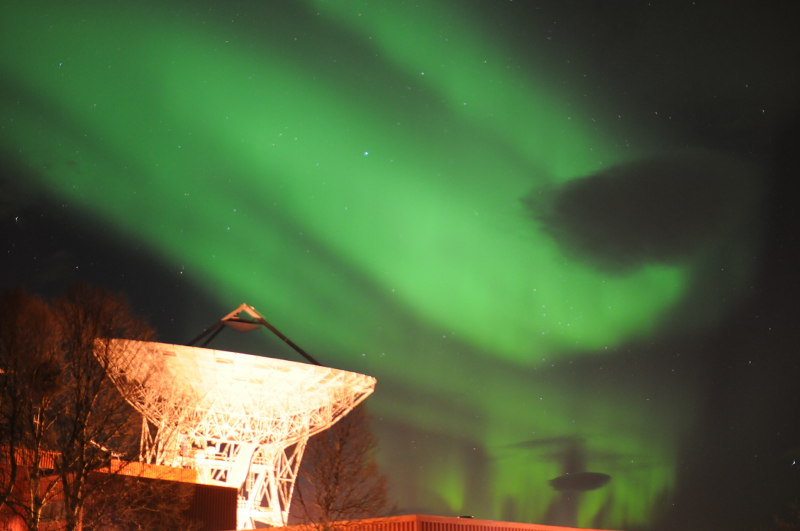
\includegraphics[height=\picsize]{uhf-tro-aurora.jpg}
% 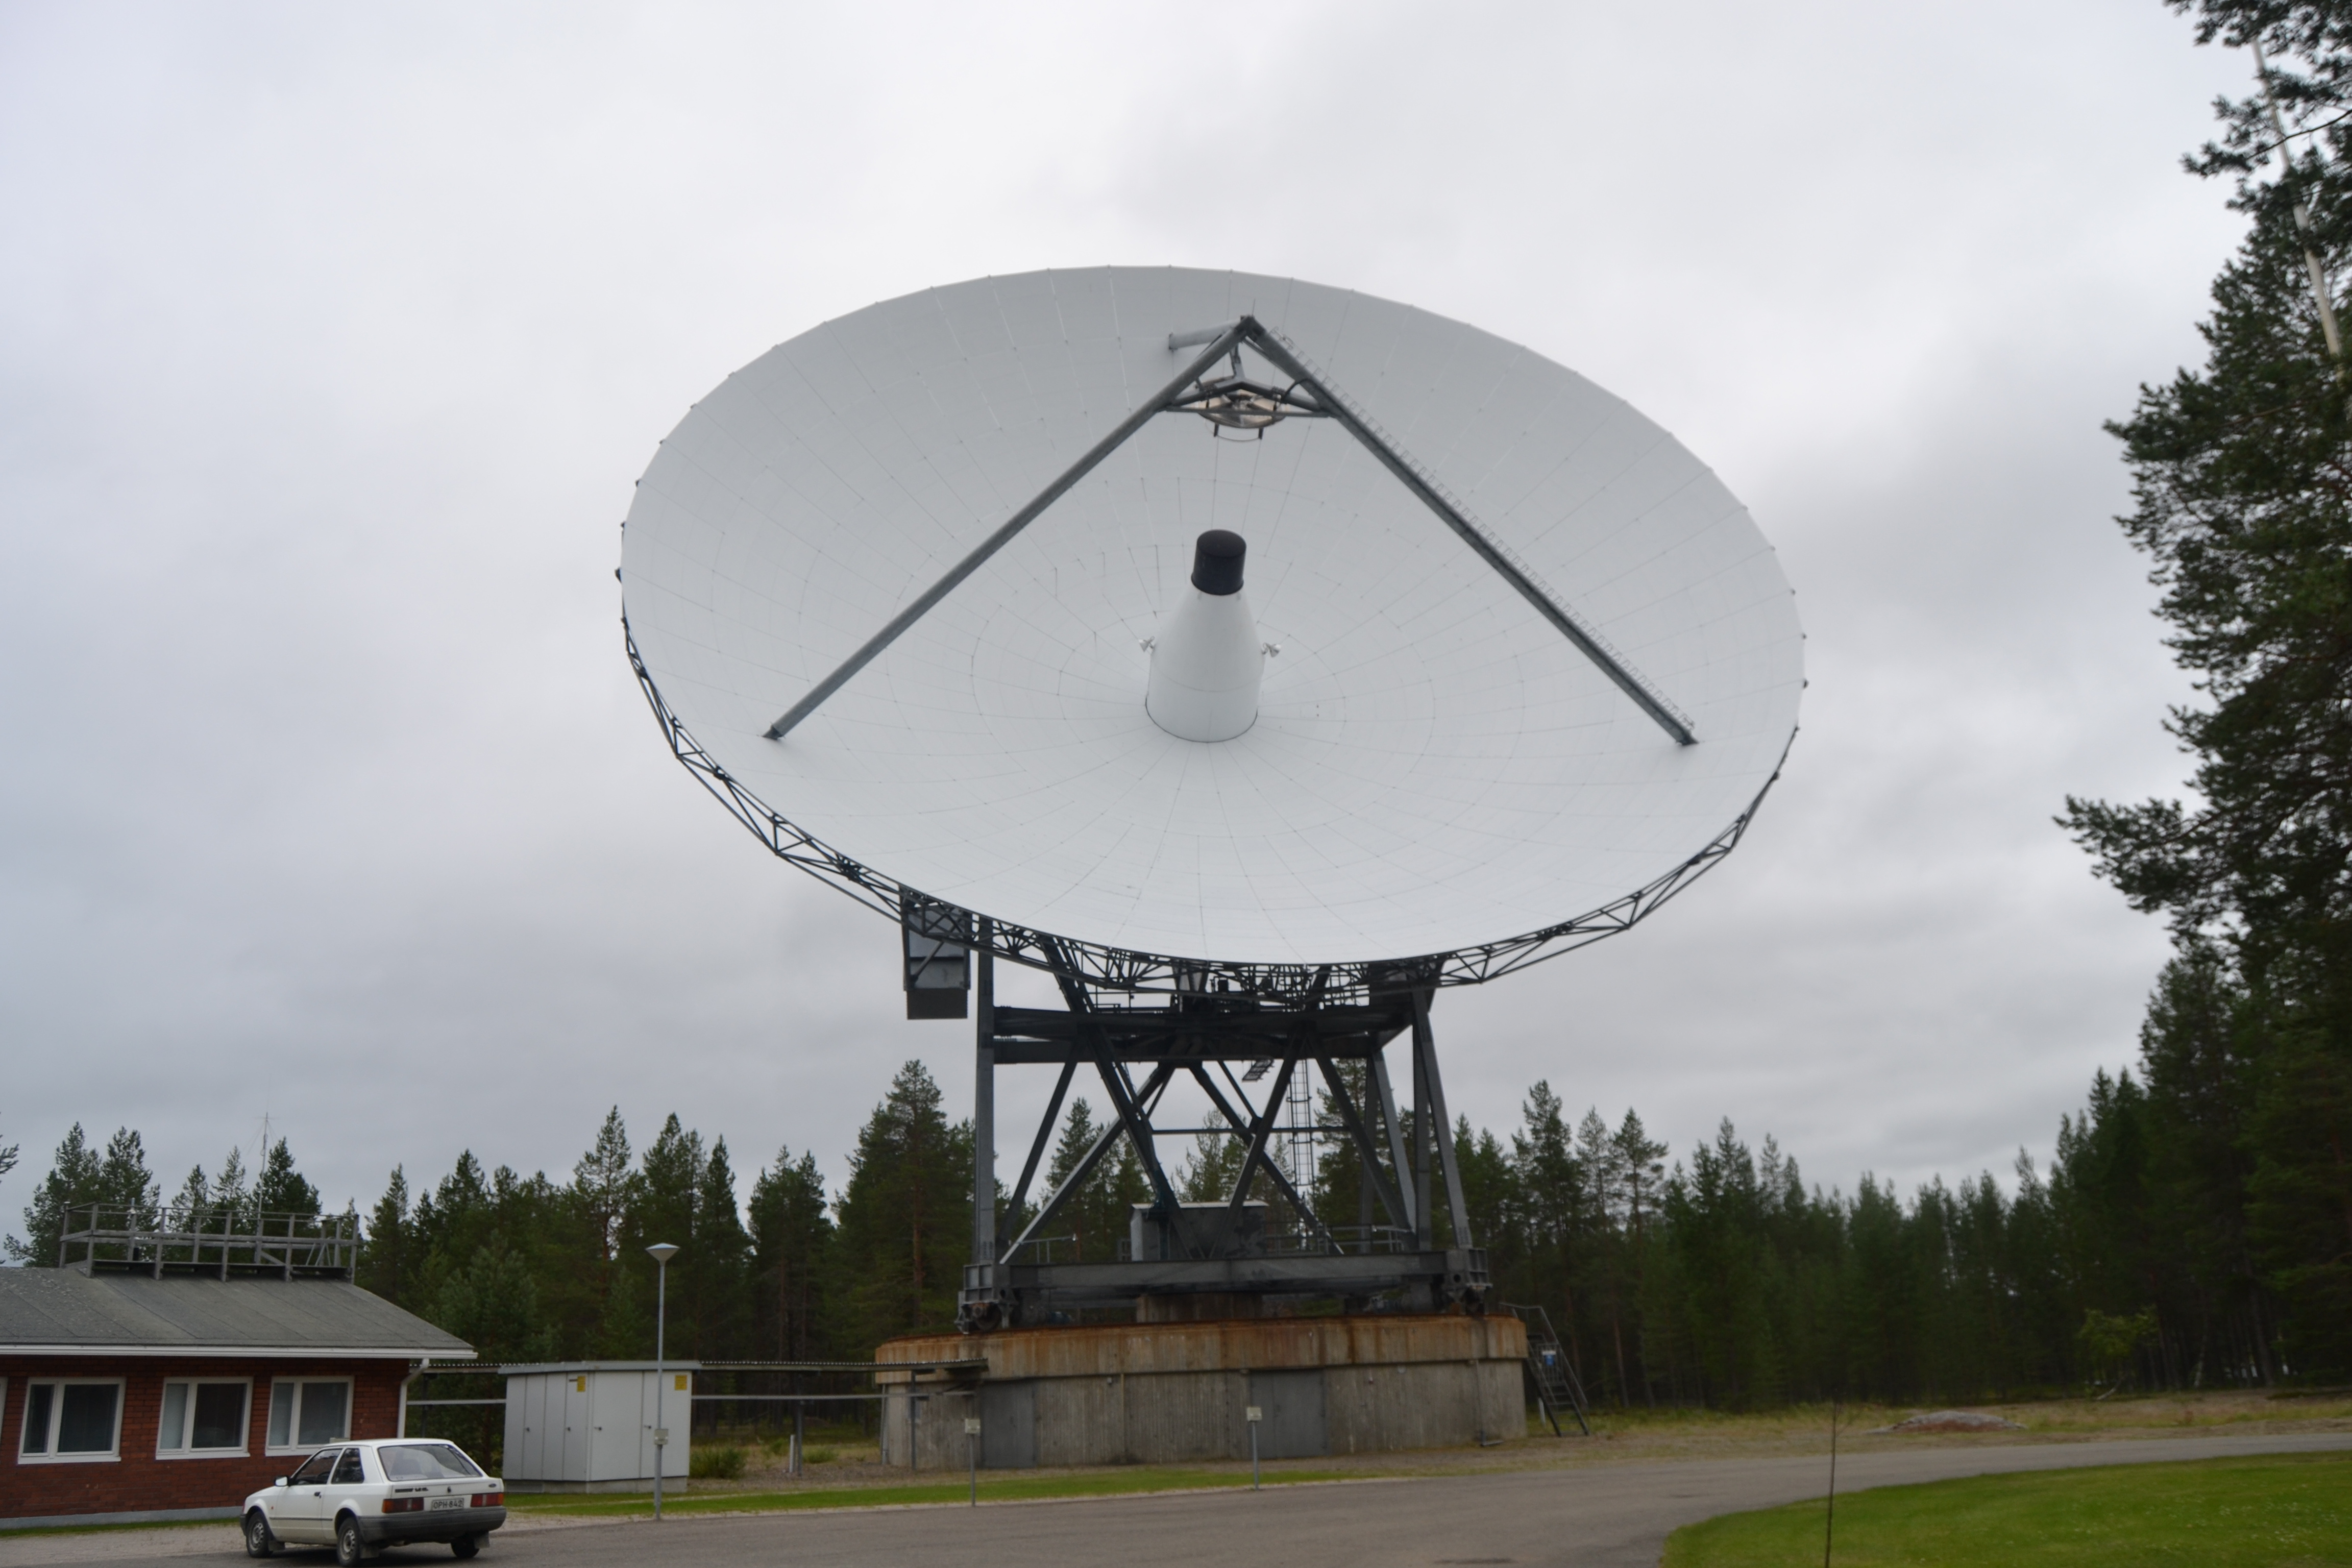
\includegraphics[height=\picsize]{EISCAT_Sodankyla_radar.jpg}
% 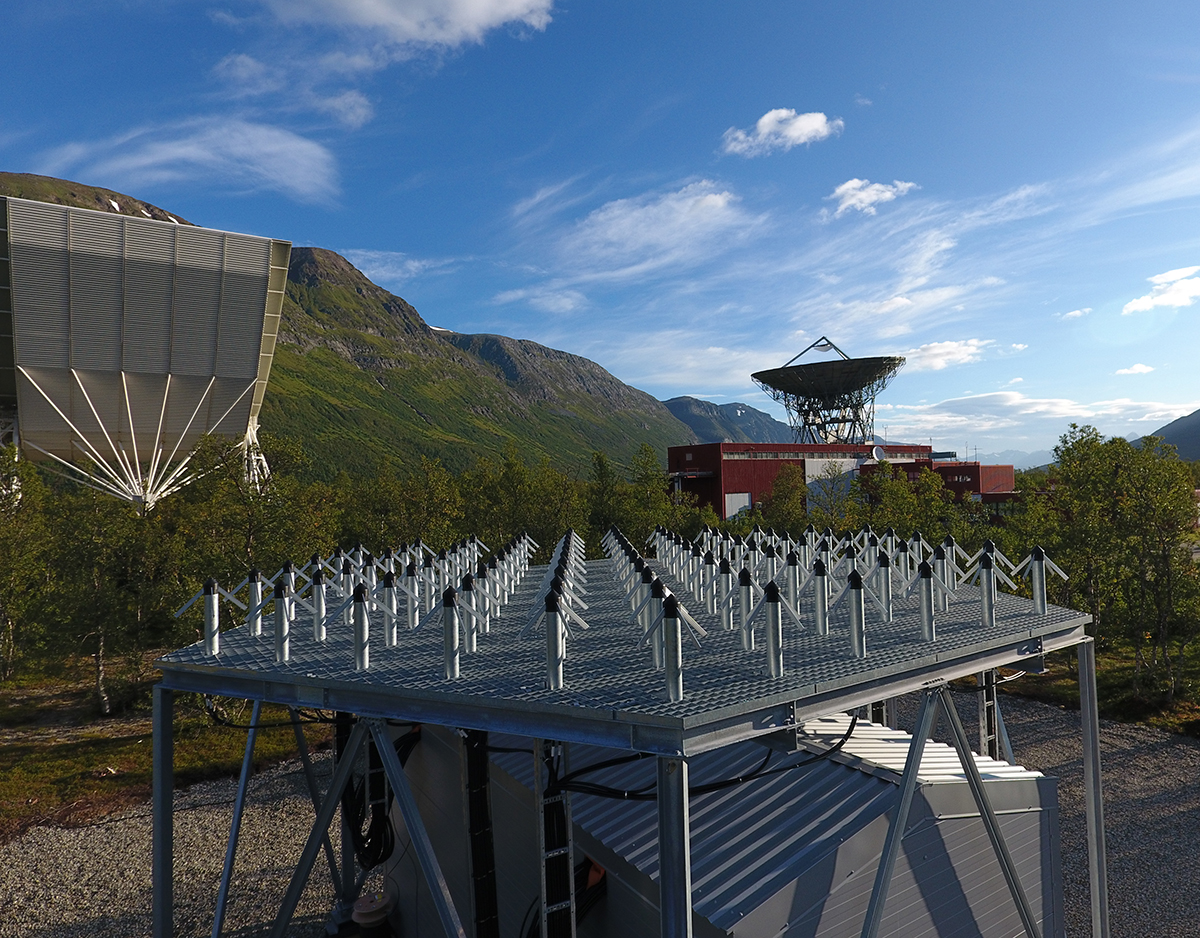
\includegraphics[height=\picsize,width=1.95in]{Tromso-eiscat3d.jpg}
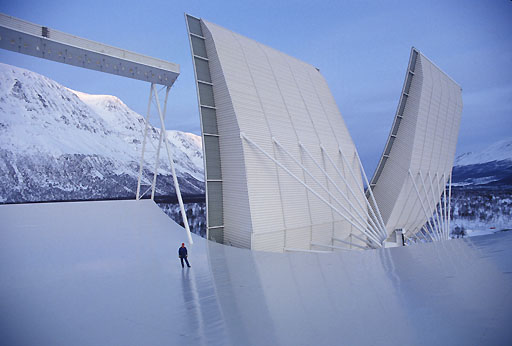
\includegraphics[height=\picsize,width=1.95in]{eiscat-vhf.jpg}

{\scriptsize Troms{\o} UHF monostatic 930 MHz 69$^\circ$ N \hfill VHF tristatic 224 MHz}

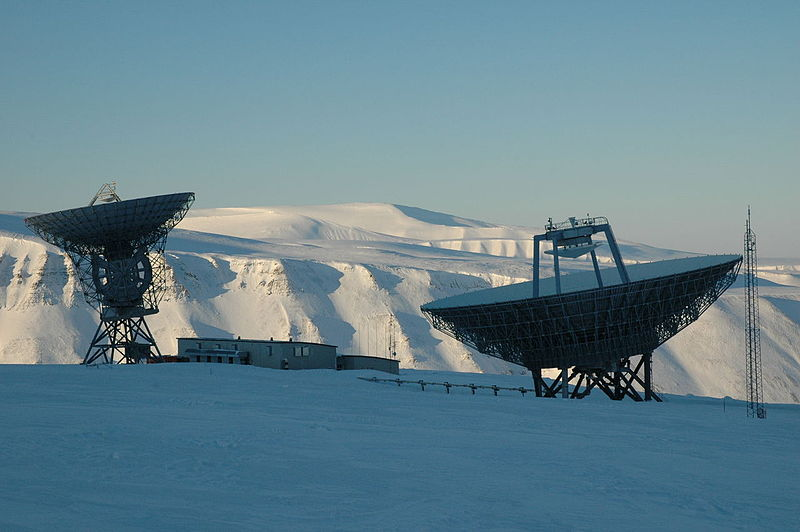
\includegraphics[height=\picsize]{EISCAT_Svalbard_Radar.jpg}
                \raisebox{1.2cm}{
                \begin{minipage}{0.46\textwidth}
                \begin{itemize}
                    \item {\colblack Campaign operation using to fixed schedules.}
                    \item {\colblack Oldest system since 1981.}
                    \item {\colblack Dataset since 1981 $<100$~TB.}
                \end{itemize}
                {\colblack \scriptsize \it NASA via Wikimedia Commons, EISCAT}
                
                \end{minipage}
            }
 
  {\scriptsize Svalbard dual antenna 500 MHz 78$^\circ$ N \hfill}          
}
\end{center}
\vfill
    {\colblack {\bf E}uropean {\bf I}ncoherent {\bf Scat}ter Scientific Association ({\bf EISCAT})}
    {\small \url{https://www.eiscat.se/}}
\end{frame}

